\documentclass[12pt]{article}
\usepackage[letterpaper,margin={1.5cm}]{geometry}
\usepackage{amsmath, amssymb, amsfonts}
\usepackage[utf8]{inputenc}
\usepackage[T1]{fontenc}
\usepackage[spanish]{babel}
\usepackage{tikz}
\usepackage{graphicx,enumitem}
\usepackage{multicol}
\setlength{\marginparsep}{12pt} \setlength{\marginparwidth}{0pt} \setlength{\headsep}{.8cm} \setlength{\headheight}{15pt} \setlength{\labelwidth}{0mm} \setlength{\parindent}{0mm} \renewcommand{\baselinestretch}{1.15} \setlength{\fboxsep}{5pt} \setlength{\parskip}{3mm} \setlength{\arraycolsep}{2pt}
\renewcommand{\sin}{\operatorname{sen}}
\newcommand{\N}{\ensuremath{\mathbb{N}}}
\newcommand{\Z}{\ensuremath{\mathbb{Z}}}
\newcommand{\Q}{\ensuremath{\mathbb{Q}}}
\newcommand{\R}{\ensuremath{\mathbb{R}}}
\newcommand{\C}{\ensuremath{\mathbb{C}}}
\newcommand{\I}{\ensuremath{\mathbb{I}}}
\graphicspath{{../imagenes/}{imagenes/}{..}}
\allowdisplaybreaks{}
\raggedbottom{}
\setlength{\topskip}{0pt plus 2pt}
\newcommand{\profesor}{Edward Y. Villegas}
\newcommand{\asignatura}{M\'ETODOS NUM\'ERICOS}
\newcommand{\diff}[3]{\frac{d^{#3} #1}{d#2^{#3}}}
\newcommand{\pdiff}[3]{\frac{\partial^{#3} #1}{\partial#2^{#3}}}
\newcommand{\abs}[1]{\left| #1 \right|}
\begin{document}
  \pagestyle{empty}
  \begin{minipage}{\linewidth}
    \centering
    \begin{tikzpicture}[very thick,font=\small]
      \node at (2,6) {
\includegraphics[width=3.5cm]{logoudem}};
      \node at (9.5,6) {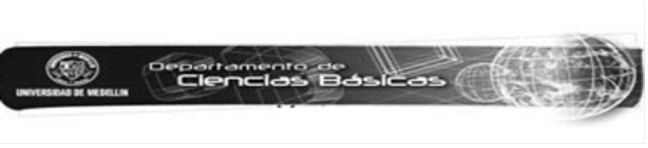
\includegraphics[width=9cm]{cbudem}};
      \node[fill=white,draw=white,inner sep=1mm] at (9.5,5.05) {\bf Permanencia con calidad, Acompa\~nar para exigir};
      \node[fill=white,draw=white,inner sep=1mm] at (7.5,4.2) {\Large\bf DEPARTAMENTO DE CIENCIAS B\'ASICAS};
      \draw (0,0) rectangle (18,3.5);
      \draw (0,2.5)--(18,2.5) (0,1.5)--(18,1.5) (15,4.2)--(18,4.2) node[below,pos=.5] {CALIFICACI\'ON} (15,2.5)--(15,7)--(18,7)--(18,3.5) (8.4,0)--(8.4,1.5) (15,0)--(15,1.5) (10,1.5)--(10,2.5);
      \node[right] at (0,3.2) {\bf Alumno:}; \node[right] at (15,3.2) {\bf Carn\'e:};
      \node[right] at (0,2.2) {\bf Asignatura:};
      \node at (6,1.95) {\asignatura};
      \node[right] at (10,2.2) {\bf Profesor:};
      \node at (15,1.95) {\profesor};
      \node[right] at (0,1.2) {\bf Examen:};
      \draw (3.8,.9) rectangle (4.4,1.3); \node[left] at (3.8,1.1) {Parcial:};
      \draw (3.8,.2) rectangle (4.4,.6); \node[left] at (3.8,.4) {Previa:};
      \draw (7.4,.9) rectangle (8,1.3); \node[left] at (7.4,1.1) {Final:};
      \draw (7.4,.2) rectangle (8,.6); \node[left] at (7.4,.4) {Habilitaci\'on:};
      \node at (4, .4) {X}; % Quiz
      \node[right] at (10,.5) {8}; % Número de grupo
      \node[right] at (10,1.) {14 de octubre de 2016}; % Fecha de presentación
      \node[right] at (8.4,1.05) {\bf Fecha:}; \node[right] at (8.4,.45) {\bf Grupo:};
      \node[align=center,text width=3cm,font=\footnotesize] at (16.5,.75) {\centering\bf Use solo tinta\\y escriba claro};
    \end{tikzpicture}
  \end{minipage}
{\scriptsize
Se permite usar calculadora de cualquier tipo mas no el uso de portátil o celulares en el examen, y puede disponer de sus apuntes de clase.
No se permite hablar ni prestar elementos durante el examen.
Todo valor reportado debe aproximarse a 5 cifras significativas con redondeo simétrico (no es necesario en enteros y valores dados en enunciado) salvo que se indique lo contrario en el enunciado, y con coma decimal.
Valide siempre las condiciones suficientes o necesarias según corresponda a cada método antes de aplicarlo, salvo que se indique lo contrario. Si algún elemento solicitado en teoría no puede realizarse, justifique por que no se puede realizar lo solicitado como respuesta. Todo procedimiento debe explicarse e indicarse su respuesta final de forma acorde al enunciado.
En caso de reclamación solo cuenta lo que este en lapicero.
Si necesita espacio adicional use el respaldo de las hojas para el procedimiento (no se permiten hojas extras) y resuelva los puntos en orden.
}
\vspace{-.5cm}
  \begin{enumerate}[leftmargin=*,widest=9]
    \item Representada la evolución temporal de la corriente eléctrica por los datos
    \begin{center}
   		\begin{tabular}{ | c | c | }
     \hline
     t (s) & I (A) \\ \hline
     $0.0$ & $0.61134$ \\ \hline
     $0.5$ & $1.0023$ \\ \hline
     $1.0$ & $1.6532$ \\ \hline
     $1.5$ & $2.7234$ \\ \hline
     $2.5$ & $7.3931$ \\
     \hline
   		\end{tabular}
 	\end{center}
   Sabemos que la carga de un capacitor viene dada por $$Q = \int_{t_i}^{t_f} I dt$$ Use integración numérica con criterio de máxima precisión para obtener la carga del capacitor
   \begin{enumerate}[label=\alph*]
    \item (\(0.5\)) ¿Que métodos / formas debe aplicar y cuantas veces?

\textbf{R/} Dado a los 4 intervalos presentes y cumpliendo criterio de máxima precisión, es necesario usar una vez el método de Simpson 3/8 simple (3 intervalos) y una vez el método del trapecio simple. Es necesario que el orden de aplicación sea justo este, ya que el último intervalo presenta una separación de puntos diferente a los primeros 3 intervalos.
    \item (\(1.0\)) Calcule la carga por integración numérica con la forma que describió en el literal anterior.

\textbf{R/} La integral solicitada puede resolverse como la suma de integrales en los dos tramos definidos para cada uno de los métodos y luego sumar su resultado. Es necesario notar que la separación de puntos para el primer tramo es de \(h=0.5s\) mientras que para el segundo tramo es de \(h=1s\).
\begin{eqnarray*}
\int_{0.0}^{2.5}Idt &=& \int_{0.0}^{1.5}Idt + \int_{1.5}^{2.5}Idt \\
\int_{0.0}^{1.5}Idt &\approx & \frac{3}{8}(0.5)(0.61134 + 3(1.0023+1.6532)+2.7234)As = 2.1190As\\
\int_{1.5}^{2.5}Idt &=& \frac{1}{2}(7.3931+2.7234)As = 5.0582As\\
\int_{0.0}^{2.5}Idt &\approx & (2.1190+5.0582)As = 7.1772As
\end{eqnarray*}
La carga en el capacitor será de \(7.1772As\).
    \end{enumerate}
    \item (\(1.0\)) Determine con aproximación central de 3 puntos la tasa de cambio de la corriente en $t = 1.0 s$ (Use la tabla del punto anterior).

\textbf{R/} La tasa de cambio corresponde a la diferenciación. De esta forma, aplicamos el método de diferenciación de 3 puntos para derivadas orden 1 sobre el punto indicado. Esto implica que requerimos de un punto adelante y un punto atras, pero siendo equidistantes. La condición de equidistantes evita que se pueda tomar los extremos ya que la distancia de ambos puntos al solicitado es distinta.
\[
\left.\diff{I}{t}{}\right|_{t=1.0s} = \frac{2.7234-1.0023}{2\cdot 0.5} \frac{A}{s} = 1.7211 \frac{A}{s}
\]
La tasa de cambio de la corriente es de \(1.7211 \frac{A}{s}\).
   \item (\(1.5\)) Dados los vertices de un dominio D,
   	\begin{eqnarray*}
   	P_1 &=& (0 , 1) \\ P_2 &=& (0 , 0.5) \\ P_3 &=& (1 , 0.8) \\ P_4 &=& (-1 , 0.7)
   	\end{eqnarray*}
Determine la integral aproximada con dos elementos triangulares de $$\iint _{D} |x-y| dx dy$$

\textbf{R/} El primer paso que requerimos para la integración de varias variables por medio de elementos finitos, es la construcción de la matriz de nodos. Esta se construye a partir de la información dada de los puntos que conocemos en la frontera del dominio.
\[
\begin{array}{cc}
0 & 1\\
0 & 0.5\\
1 & 0.8\\
-1 & 0.7
\end{array}
\]
Trabajaremos los nodos con convención de indice desde cero, pero es equivalente si el conteo empieza desde uno.
A continuación, dado que se solicitaron dos triángulos, estos pueden construirse con dicha matriz de nodos (no se requieren puntos interiores, de otra forma serían más de dos triángulos), y podemos obtener la siguiente matriz de elementos con separación vertical de los triángulos.
\[
\begin{array}{ccc}
1 & 2 & 0\\
1 & 0 & 3
\end{array}
\]
También es posible seleccionar la siguiente matriz de elementos con separación horizontal de los triángulos.
\[
\begin{array}{ccc}
3 & 2 & 0\\
3 & 1 & 2
\end{array}
\]
La orientación de los triángulos debe ser siempre antihoraria para ser valida.
Sobre cada uno de los elementos se resuelve la aproximación de la integral, como el volumen del prisma truncado, siendo el área de la base dada por la formula de Herón y la altura como el promedio de la función evaluada en los 3 vértices del triangulo, valores que se deben multiplicar.
Así, para la separación vertical tenemos:
\begin{eqnarray*}
\Delta V_0 &=& 0.25000 \frac{0.50000+0.200000+1}{3} = 0.14167\\
\Delta V_1 &=& 0.25000 \frac{0.50000+1+1.7000}{3} = 0.26667\\
\iint_D |x-y|\,dx\,dy &\approx & \Delta V_0 + \Delta V_1 = 0.40834
\end{eqnarray*}
    \item Si se conoce la evaluación de una función y su derivada en cuatro puntos,
   \begin{enumerate}[label=\alph*]
    \item (\(0.7\)) ¿Que método de interpolación debe usar?

\textbf{R/} El método de polinomios interpolantes de Hermite permite la aproximación para estos casos en los cuales se conoce no solo la evaluación de la función sino también la evaluación de la derivada de la posición en los mismos puntos.
    \item (\(0.3\)) ¿Cual es el grado de dicho polinomio interpolante?

\textbf{R/} Al tener 4 puntos y los polinomios ser de la forma \(H_{2n+1}(x)\), sabemos que
	\begin{eqnarray*}
	n + 1 &=& 4\\
	n = 3 \\
	2n + 1 &=& 2(3)+1 = 7
\end{eqnarray*}
    \end{enumerate}
\end{enumerate}
\end{document}
